\documentclass[10pt,a4paper]{article}

% --- Sprache und Schrift ---
\usepackage{fontspec}
\usepackage[ngerman]{babel}
\setmainfont{Latin Modern Roman}
\usepackage{microtype}

% --- Seitenlayout ---
\usepackage{geometry}
\geometry{
	top=1.35cm,
	bottom=1.45cm,
	left=1.6cm,
	right=1.6cm
}

\usepackage{parskip}
\setlength{\parindent}{0pt}
\setlength{\parskip}{0.22em}

% --- Tabellen / Grafiken ---
\usepackage{graphicx}
\usepackage{booktabs}
\usepackage{tabularx}
\usepackage{array}
\usepackage{caption}
\usepackage{float}
\captionsetup{
	font=small,
	labelfont=bf,
	skip=2pt
}

% --- Listen ---
\usepackage{enumitem}
\setlist[itemize]{
	leftmargin=1.2em,
	itemsep=0.12em,
	topsep=0.12em,
	parsep=0pt,
	partopsep=0pt
}

% --- Links ---
\usepackage[hidelinks]{hyperref}

% --- Abschnittsabstände kompakter machen ---
\usepackage{titlesec}
\titlespacing*{\section}{0pt}{0.45em}{0.25em}

% --- Float-Abstände kompakter ---
\setlength{\textfloatsep}{8pt plus 2pt minus 2pt}
\setlength{\floatsep}{6pt plus 2pt minus 2pt}
\setlength{\intextsep}{6pt plus 2pt minus 2pt}

% --- Kleine Format-Helfer ---
\newcommand{\reporttitle}{Technischer Kurzbericht: Auswirkungen zusätzlicher EV-Ladeleistungen auf ein Niederspannungsnetz}
\newcommand{\reportsubtitle}{Szenariobasierte Lastflussanalyse mit Python und pandapower}

\begin{document}
	
	{\Large\bfseries \reporttitle \par}
	\vspace{0.15em}
	{\normalsize \reportsubtitle \par}
	\vspace{0.2em}
	{\small Portfolio-Projekt \textbar\ Repräsentatives Kerber-Dorfnetz \textbar\ Stand: April 2026 \par}
	
	\vspace{0.3em}
	\hrule
	\vspace{0.35em}
	
	\section*{1. Kurzfassung}
	
	Dieses Dokument fasst ein technisches Portfolio-Projekt zur Bewertung zusätzlicher EV-Ladeleistungen in einem repräsentativen Niederspannungsnetz zusammen. Untersucht werden die Auswirkungen unterschiedlicher EV-Szenarien auf Transformatorauslastung, Leitungsauslastung und minimale Knotenspannung auf Basis stationärer Lastflussrechnungen mit Python und pandapower. Ergänzend werden eine vereinfachte netzorientierte Leistungsbegrenzung sowie eine Grenzpenetrationsanalyse eingesetzt, um sowohl die Wirkung einer einfachen Gegenmaßnahme als auch die erste kritische EV-Aufnahmegrenze abzuschätzen. Die Ergebnisse zeigen, dass der Transformator im betrachteten Netz den dominanten Engpass darstellt und dass eine Reduktion der Wallbox-Leistung die technische Situation verbessert, kritische Zustände jedoch nicht vollständig beseitigt.
	
	\section*{2. Netzmodell und methodisches Vorgehen}
	
	Als Netzmodell wird das repräsentative Niederspannungs-Testnetz \texttt{create\_kerber\_dorfnetz()} aus \texttt{pandapower} verwendet. Es handelt sich nicht um ein reales Versorgungsgebiet, sondern um ein typisches Referenznetz für eine nachvollziehbare und reproduzierbare Portfolioanalyse. Im Mittelpunkt steht dabei nicht die Abbildung eines konkreten Netzbetreibergebiets, sondern die systematische Bewertung relativer Veränderungen zwischen Referenzfall, EV-Szenarien, Mitigation und Grenzpenetration.
	
	\begin{itemize}
		\item Stationäre Lastflussberechnung für die Szenarien S0 bis S3
		\item Bewertung von Transformatorauslastung, maximaler Leitungsauslastung und minimaler Knotenspannung
		\item Vereinfachter Mitigationstest durch Reduktion der Wallbox-Leistung von 11\,kW auf 7\,kW im Stressfall
		\item Grenzpenetrationsanalyse zur Abschätzung der ersten kritischen EV-Aufnahmegrenze unter konstanten Annahmen
	\end{itemize}
		
	\section*{3. Zentrale Kennzahlen}
	
	\begin{table}[H]
		\centering
		\footnotesize
		\begin{tabularx}{\textwidth}{>{\raggedright\arraybackslash}X >{\raggedleft\arraybackslash}p{4.0cm}}
			\toprule
			\textbf{Kennzahl} & \textbf{Ergebnis} \\
			\midrule
			Transformatorauslastung im Stressfall (S3) & 231,2 \% \\
			Maximale Leitungsauslastung im Stressfall (S3) & 153,6 \% \\
			Minimale Knotenspannung im Stressfall (S3) & 0,8631 pu \\
			Trafo-Auslastung S3 $\rightarrow$ S3-M (7 kW) & 231,2 \% $\rightarrow$ 176,8 \% \\
			Erste kritische EV-Penetration ohne Mitigation & ca.\ 12 \% \\
			Erste kritische EV-Penetration mit 7-kW-Mitigation & ca.\ 18 \% \\
			\bottomrule
		\end{tabularx}
	\end{table}
	
	\section*{4. Zentrale Ergebnisse der Szenarioanalyse}
	
Die Szenarioanalyse zeigt eine klare Zunahme der Netzbeanspruchung mit steigender EV-Integration. Besonders deutlich wird dies bei der Transformatorauslastung, die vom Referenzfall über die EV-Szenarien hinweg stark ansteigt und im Stressfall einen ausgeprägt kritischen Bereich erreicht. Parallel dazu nehmen auch die Leitungsauslastungen zu, während das Spannungsniveau im Netz sichtbar absinkt. Im betrachteten Referenznetz ist der Transformator damit als maßgebender Engpass einzuordnen, während die Leitungen im Stressfall ebenfalls technisch relevante Zusatzbelastungen aufweisen.
	
	\begin{figure}[H]
		\centering
		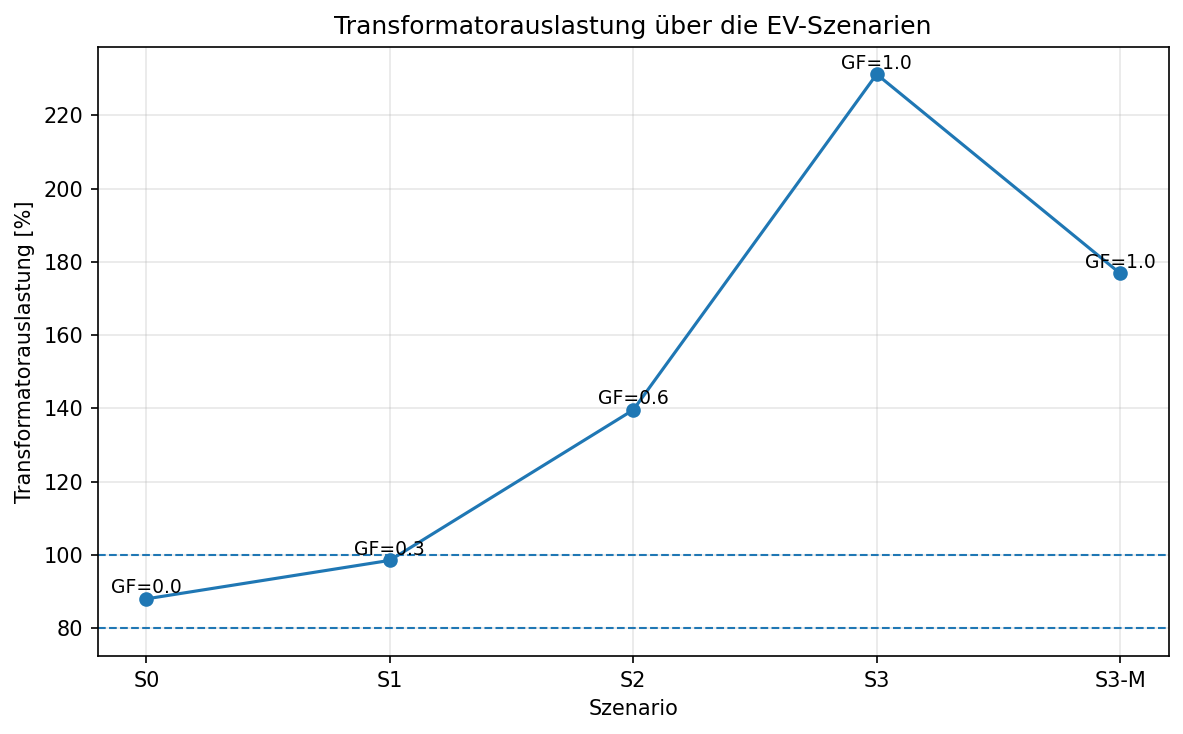
\includegraphics[width=0.66\textwidth]{../figures/transformatorauslastung_szenarien.png}
		\caption{Transformatorauslastung über die betrachteten Szenarien.}
	\end{figure}
	
	\section*{5. Mitigation und Grenzpenetration}
	
Der vereinfachte Mitigationstest zeigt, dass eine Reduktion der Wallbox-Leistung die technische Belastung im Stressfall spürbar senken kann. Insbesondere verbessern sich Transformatorauslastung, Leitungsauslastung und Spannungsniveau gegenüber dem ursprünglichen Stressszenario, ohne jedoch einen vollständig unkritischen Betriebszustand zu erreichen. Ergänzend verdeutlicht die Grenzpenetrationsanalyse, dass sich die erste kritische EV-Aufnahmegrenze durch die Mitigation nach oben verschiebt. Damit zeigt das Projekt nicht nur die Belastungswirkung zusätzlicher EV-Ladeleistungen, sondern auch den technischen Nutzen einer einfachen netzorientierten Gegenmaßnahme.
	
	\begin{figure}[H]
		\centering
		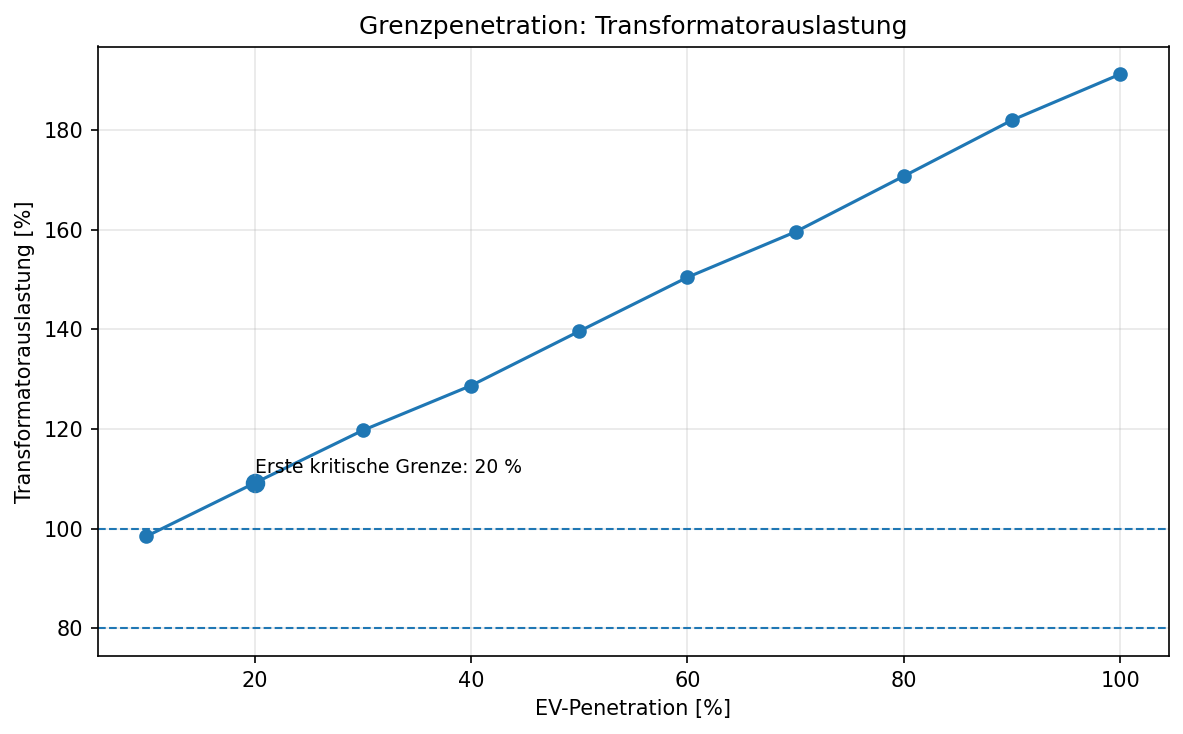
\includegraphics[width=0.66\textwidth]{../figures/grenzpenetration_trafo_baseline.png}
		\caption{Grenzpenetration in Bezug auf die Transformatorauslastung.}
	\end{figure}
	
	\section*{6. Grenzen der Analyse}
	
	\begin{itemize}
		\item Verwendung eines repräsentativen Testnetzes statt eines real kalibrierten Versorgungsgebiets
		\item Stationäre Lastflussanalyse ohne zeitliche Lastprofile oder Zeitreihensimulation
		\item Vereinfachte technische Bewertungslogik zur Einordnung der Ergebnisse, kein formaler Netznachweis nach projektspezifischen Betreiberregeln
	\end{itemize}
	
	\section*{7. Fazit}
	
	Das Projekt zeigt, dass zusätzliche EV-Ladeleistungen bereits in einem vereinfachten Niederspannungsnetz zu deutlich erhöhten technischen Belastungen führen können. Im betrachteten Referenznetz ist der Transformator der dominierende Engpass, während im Stressfall auch die Leitungen und das Spannungsniveau zunehmend kritisch werden. Die vereinfachte Leistungsbegrenzung verbessert die technische Situation und verschiebt die geschätzte kritische Aufnahmegrenze nach oben, beseitigt die bestehenden Netzprobleme jedoch nicht vollständig. Insgesamt liefert das Projekt damit eine kompakte und nachvollziehbare technische Argumentation aus Szenariovergleich, vereinfachter Gegenmaßnahme und Grenzabschätzung.
	
\end{document}